% !TeX root = ../../Report.tex
% !TeX encoding = UTF-8
در این پوشه به ارتباط با پایگاه‌داده پرداخته می‌شود و تمام اطلاعات از پایگاه داده واکشی می‌شود.

\begin{figure}[H]
	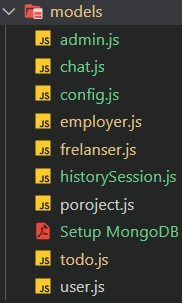
\includegraphics[width=.3\textwidth]{Folders-Files/models.png}
	\centering
	\caption{ساختار پوشه مدل}
	\label{fig:folder-models}
\end{figure}

\subsection{فایل user}
در این فایل به ارسال و دریافت اطلاعات کاربر شامل اسم، اطلاعات کاربری، رمز، نشست‌ها و ... از پایگاه‌داده پرداخته شده است.

\subsection{فایل employer}
در این فایل به ارسال و دریافت اطلاعات داشبورد کارفرما از پایگاه‌داده پرداخته شده است.

\subsection{فایل frelanser}
در این فایل به ارسال و دریافت‌اطلاعات داشبورد فریلنسر از پایگاه‌داده پرداخته شده است.

\subsection{فایل admin}
در این فایل به ارسال و دریافت‌اطلاعات داشبورد مدیریت از پایگاه‌داده پرداخته شده است.

\subsection{فایل chat}
در این فایل به ارسال و دریافت پیام‌های ‌داخلی که شامل ارتباط کارفرما و فریلنسر، ارتباط کارفرما و مدیریت، ارتباط مهمان و مدیریت، ... از پایگاه‌داده پرداخته شده است.

\subsection{فایل config}
در این فایل به ارسال و دریافت تنظیمات عمومی از پایگاه‌داده پرداخته شده است.

\subsection{فایل project}
در این فایل به ارسال و دریافت اطلاعات پروژه از پایگاه‌داده پرداخته شده است.

\subsection{فایل todo}
در این فایل به ارسال و دریافت لیست کار از پایگاه‌داده پرداخته شده است.

